% new tcolorbox environment
\newtcolorbox{topQuark}[2][]{
  coltext      = black,
  colframe     = \MyBlockFrameColorLeft,
  colback      = \MyBlockFillColorLeft,
  colbacktitle = \MyBlockTitleBoxColor,
  coltitle     = black,
  title        = {\Large{\textbf{#2}}},
  fonttitle    = \bfseries,
  boxrule      = 0.2cm, %frame line width
  %tikz={rotate=#3}, % manipulate the tcolorbox as a whole (in degrees)
  top=+0.0cm, bottom=+0.0cm, left=+0.05cm, right=+0.05cm,
  %enlarge top by   = +1.0cm,  %  equivalent to mdframed 'skipabove'
  %enlarge bottom by= +0.0cm,  %  equivalent to mdframed 'skipbelow'
  %enlarge left by  = +1.5cm,  
  %enlarge right by = +0.0cm, 
  opacityback=1.0, % 1.0 means totally transparent, 0.0 means totally opaque
  arc=0.0cm,        % 0.0cm for non-rounded corners!
  #1,
}


\begin{topQuark}[enhanced, tikz={rotate=0}]{Top Quark, Last Piece of Matter, Appears to Be in Place}
  \begin{multicols}{2}
    We establish the existence of the top quark using a 67 pb$^{-1}$ data
    sample of pp collisions at $\sqrt{s} = 1.8$ TeV collected with the Collider
    Detector at Fermilab (CDF). Employing techniques similar to those we
    previously published, we observe a signal consistent with $t\bar{t}$ decay to
    $WWbb$, but inconsistent with the background prediction by
    4.8$\sigma$. Additional evidence for the top quark is provided by a peak in
    the reconstructed mass distribution. We measure the top quark mass
    to be $176 \pm 8 (\text{stat.}) \pm 10 (\text{sys.})$ GeV/c$^{2}$,
    and the $t\bar{t}$ production cross section to be
    $6.8^{+3.6}_{-2.4}$ pb.
    % ========================
    \begin{figure}
      \begin{center}
        \vspace{-0.2in}
        \leavevmode
        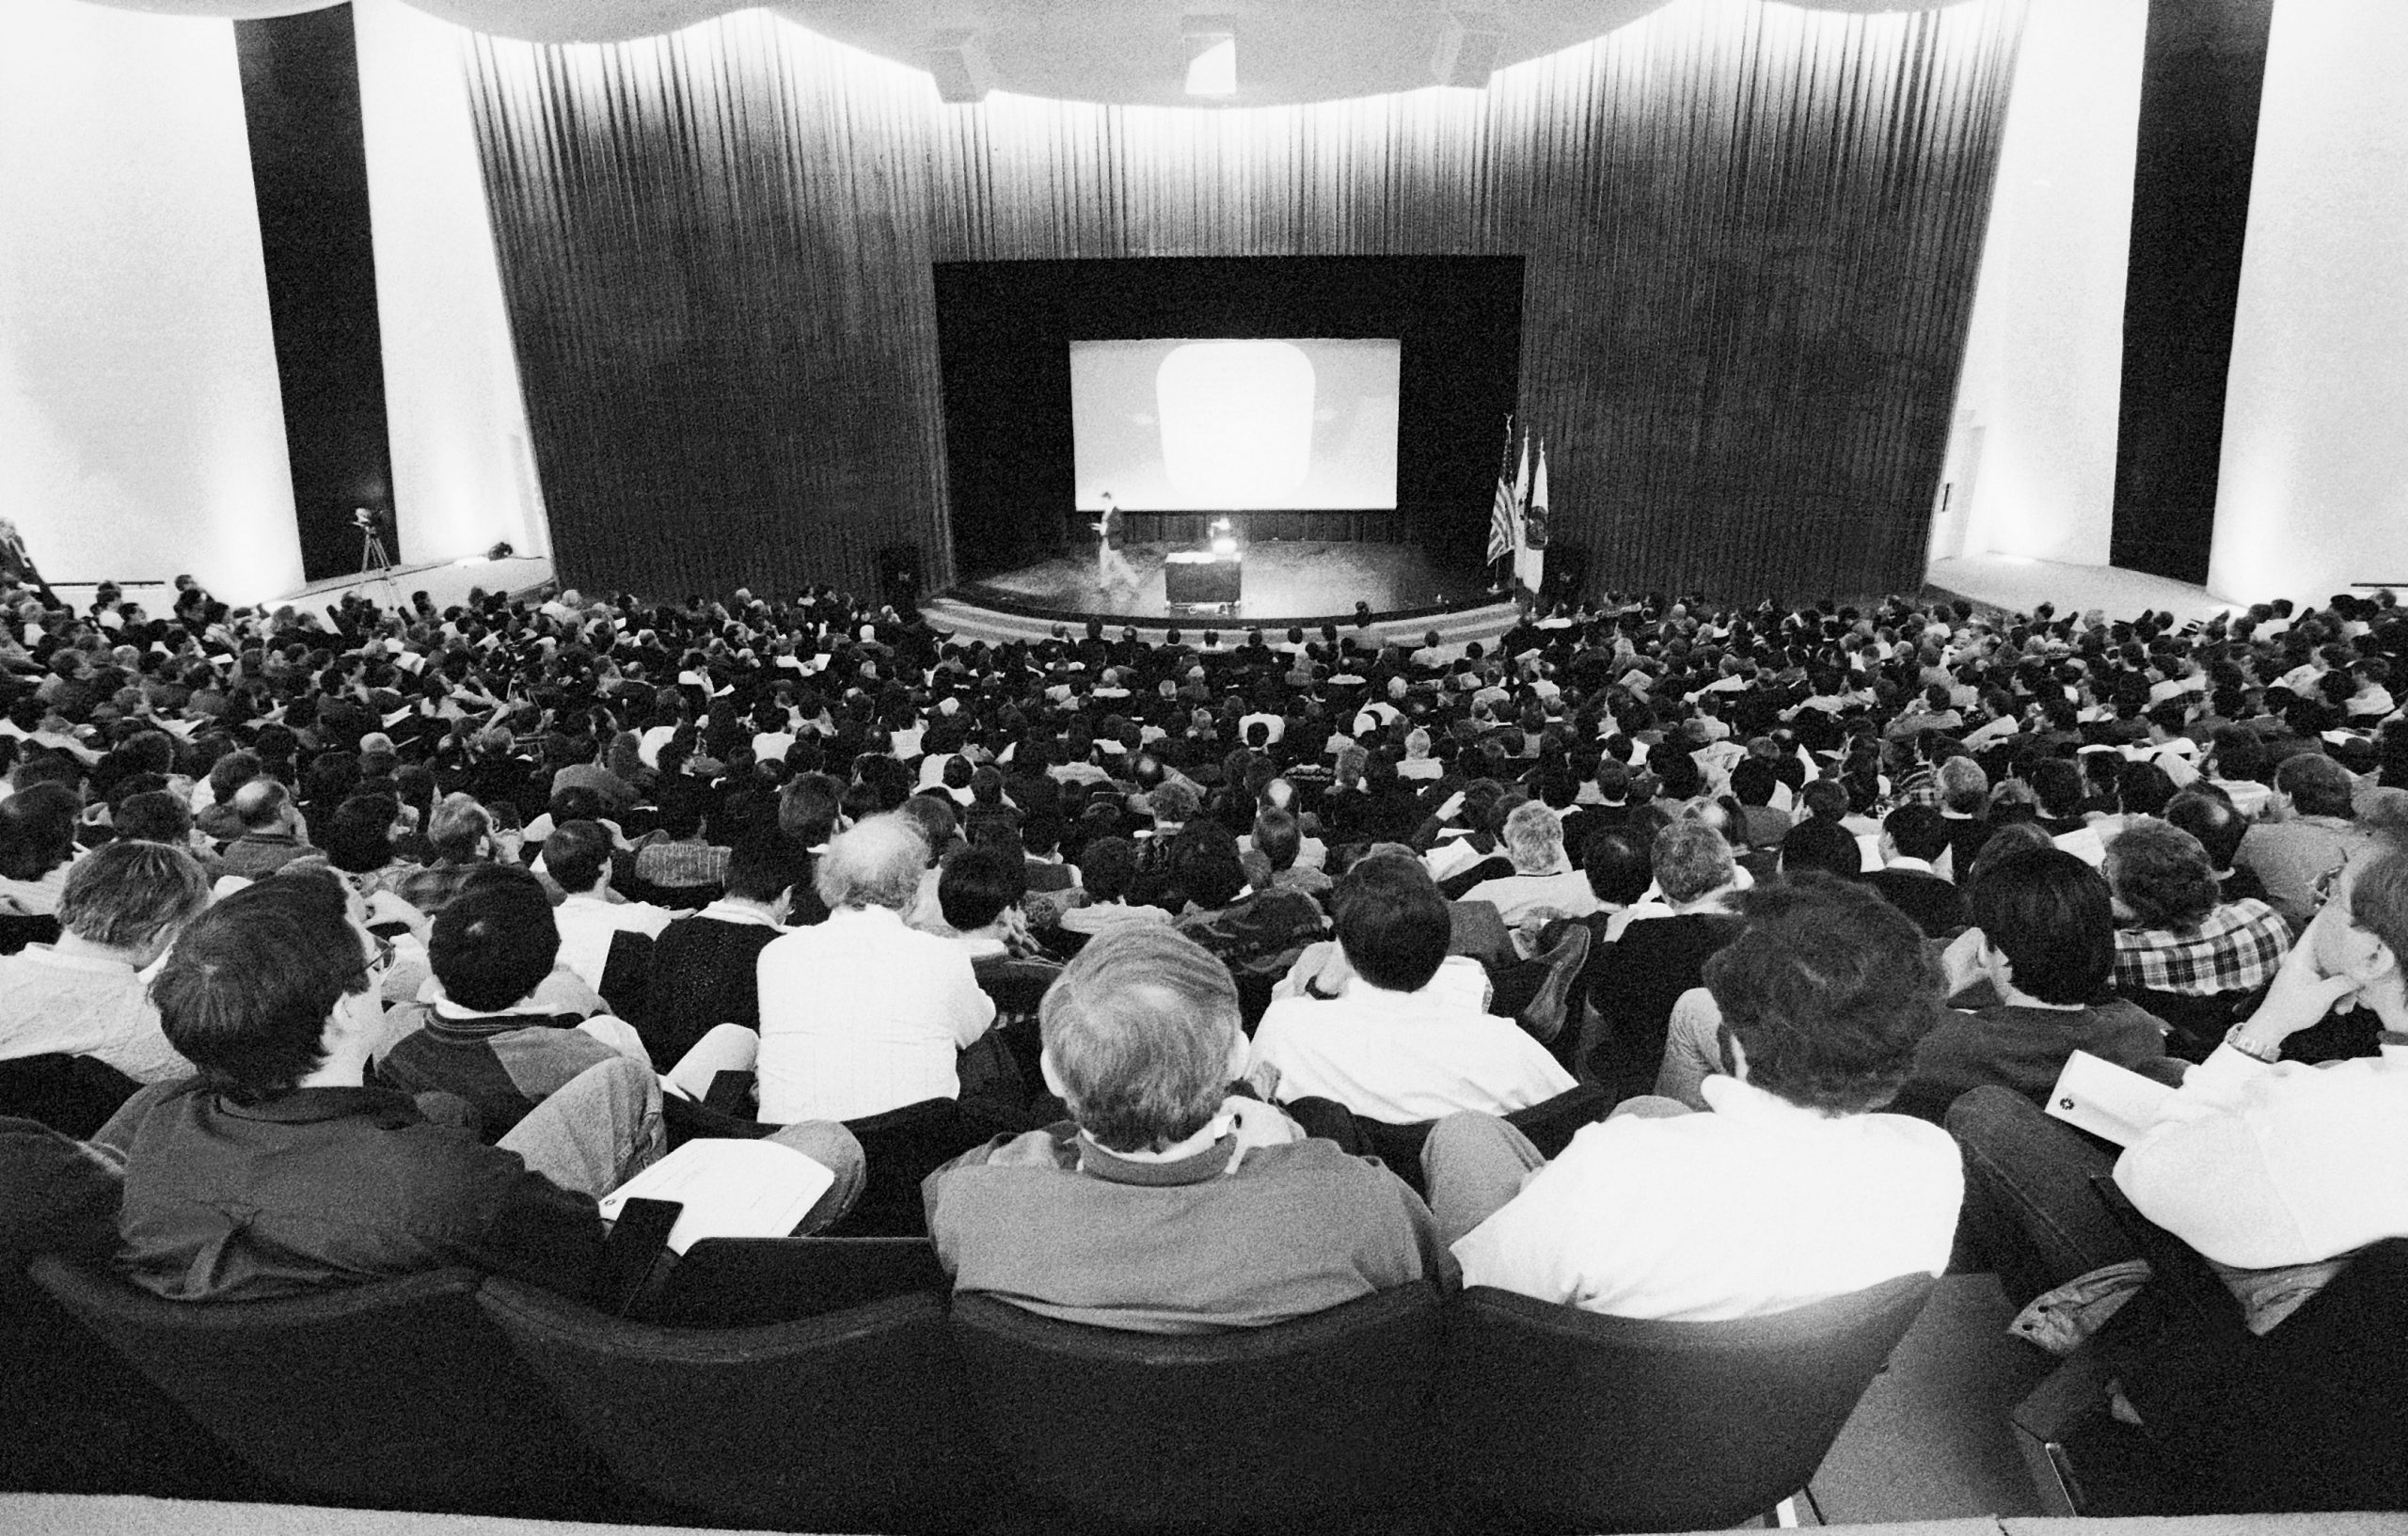
\includegraphics[width=0.5\textwidth]{./figures/TopQuarkAnnouncement.jpg}
      \end{center}
    \end{figure}
    % ========================
  \end{multicols}
\end{topQuark}
